%beamer

%\PassOptionsToClass{handout}{beamer}

% \newboolean{handoutmode}
% \setboolean{handoutmode}{false}
%\newcommand{\handoutmode}{}

%% LaTeX-Beamer template for KIT design
%% by Erik Burger, Christian Hammer
%% title picture by Klaus Krogmann
%%
%% version 2.1
%%
%% mostly compatible to KIT corporate design v2.0
%% http://intranet.kit.edu/gestaltungsrichtlinien.php
%%
%% Problems, bugs and comments to
%% burger@kit.edu
\ifdefined \handoutmode
\documentclass[18pt, handout]{beamer}
\else
\documentclass[18pt]{beamer}
\fi

\usepackage[T1]{fontenc}
\usepackage[utf8]{inputenc}

\usepackage{../preamble/templates/beamerthemekit}

\usepackage[vlined]{algorithm2e}  %possible: noend, noline, ...
\usepackage{amssymb}
\usepackage{amsmath}
\usepackage{wasysym}
\usepackage{graphicx}
%\usepackage{hyperref}
\usepackage[export]{adjustbox}
\usepackage{wrapfig}
\usepackage{colortbl}
\usepackage{tikz}
\usetikzlibrary{matrix}
\usetikzlibrary{arrows.meta}
\usetikzlibrary{automata}
\usetikzlibrary{tikzmark}
\graphicspath{{images/}}
%\usepackage[colorlinks=true,urlcolor=blue,linkcolor=blue]{hyperref}
\usepackage[outline]{contour}
\usepackage{cancel}
\usepackage[warn]{textcomp}
\usepackage{multicol}
\usepackage{tabularx}
\usepackage{xcolor}
\usepackage{hhline}
\usepackage{environ}
\usepackage{calc}
\usepackage{bm}
\usepackage{xspace} % for \xspace command
\usepackage{varwidth}
\usepackage{csquotes}

\newcommand{\mycomment}[1]{}

%%%% CONFIG

\input{../preamble/config.tex}

%%%% CONFIG END

%\renewcommand{\SS}{\iffontchar\font"1E9E \symbol{"1E9E}\else SS\fi} % SHAME ON YOU, LATEX!
\newcommand{\TM}{\text{$\mbox{}^\text{\tiny TM}$}}
\newcommand{\pluseq}{\mathrel{+}=}
\newcommand{\pp}{\operatorname{++}} 
\newcommand{\mm}{\operatorname{--\mbox{\:}--}}
\newcommand{\minuseq}{\mathrel{-}=}
\newcommand{\asteq}{\mathrel{*}=}
\newcommand{\muleq}{\asteq}
\renewcommand{\mod}{\mathop{\textbf{mod}}} 
\renewcommand{\div}{\mathop{\textbf{div}}}
\newcommand{\N}{\mathbb{N}} 
\newcommand{\R}{\mathbb{R}}
\newcommand{\Z}{\mathbb{Z}}
\newcommand{\E}{\mathbb{E}}
\renewcommand{\P}{\mathbb{P}}
\newcommand{\BB}{\mathbb{B}} % \B already exists
\newcommand{\NP}{\ensuremath{\mathcal{N\hspace{-1.5pt}P}}}
\newcommand{\Oh}[1]{\mathcal{O}\!\left(#1\right)}
\renewcommand{\O}{\mathcal{O}}
\newcommand{\Om}[1]{\Omega\!\left(#1\right)}
\newcommand{\Th}[1]{\Theta\!\left(#1\right)}

\newcommand{\realTilde}{\textasciitilde\xspace}
\renewcommand{\qedsymbol}{\textcolor{black}{\openbox}}

\newcommand{\size}[1]{\ensuremath{\left\lvert #1 \right\rvert}}
\newcommand{\set}[1]{\left\{#1\right\}}
\newcommand{\tuple}[1]{\left(#1\right)}

\newcommand*{\from}{\colon}

\newcommand{\morescalingdelimiters}{   % for proper \left( \right) typography
	\delimitershortfall=0pt  % formerly: 0pt  
	\delimiterfactor=1
}
% todo later
%\delimitershortfall=0pt  % for proper \left( \right) typography
%\delimiterfactor=1

% --- \frameheight constant ---
\newlength\fullframeheight
\newlength\framewithtitleheight
\setlength\fullframeheight{.92\textheight}
\setlength\framewithtitleheight{.86\textheight}

\newlength\frameheight
\setlength\frameheight{\fullframeheight}

\let\frametitleentry\relax
\let\oldframetitle\frametitle
\def\frametitle#1{\global\def\frametitleentry{#1}\if\relax\frametitleentry\relax\else\setlength\frameheight{\framewithtitleheight}\fi\oldframetitle{#1}}

% --- \frameheight constant end ---

\def\·{\cdot}
\def\*{\cdot}
\def\<{\langle}
\def\>{\rangle}


\newcommand{\zB}{z.\,B.\@\xspace}
\newcommand{\ZB}{Z.\,B.\@\xspace}

\newcommand{\ceil}[1]{\left\lceil#1\right\rceil}
\newcommand{\floor}[1]{\left\lfloor#1\right\rfloor}
\newcommand{\abs}[1]{\left|#1\right|}
\newcommand{\Matrix}[1]{\begin{pmatrix} #1 \end{pmatrix}}
\newcommand{\braced}[1]{\left\lbrace #1 \right\rbrace}
\newcommand{\llist}[1]{\langle #1 \rangle}
\newcommand{\Mid}{\;\middle|\;}

\let\after\circ

\newcommand{\entspr}{\ensuremath{\mathrel{\hat{=}}}\xspace}

\def\~~>{\ensuremath{\rightsquigarrow}}  % FuCKING FINALLY! :D

% "something" placeholder. Useful for repairing spacing of operator sections, like `\sth = 42`.
\def\sth{\vphantom{.}}

\def\fract#1/#2 {\frac{#1}{#2}}  % ! TRAILING SPACE is CRUCIAL!
\def\dfract#1/#2 {\dfrac{#1}{#2}} % ! Trailing space is crucial!

\newcommand{\tight}[1]{{\renewcommand{\arraystretch}{0.76} #1}}
\newcommand{\stackedtight}[1]{{\renewcommand{\arraystretch}{0.76} \begin{matrix} #1 \end{matrix}} }
\newcommand{\stacked}[1]{\begin{matrix} #1 \end{matrix} }
\newcommand{\casesl}[1]{\delimitershortfall=0pt  \left\lbrace\hspace{-.3\baselineskip}\begin{array}{ll} #1 \end{array}\right.}
\newcommand{\casesr}[1]{\delimitershortfall=0pt  \left.\begin{array}{ll} #1 \end{array}\right\rbrace}
\newcommand{\caseslr}[1]{\delimitershortfall=0pt  \left\lbrace\begin{array}{ll} #1 \end{array}\hspace{-.3\baselineskip}\right\rbrace}

\def\q#1uad{\ifnum#1=0\relax\else\quad\q{\the\numexpr#1-1\relax}uad\fi}
% e.g. \q1uad = \quad, \q2uad = \qquad etc.

\newcommand{\qqquad}{\q3uad}


\def\indentstring{}
\def\§#1{\def\indentstring{#1}#1}
\def\.{{$\hphantom{\text{\indentstring}}$}}


\newcommand{\impl}{\ifmmode\ensuremath{\mskip\thinmuskip\Rightarrow\mskip\thinmuskip}\else$\Rightarrow$\xspace\fi}  
\newcommand{\Impl}{\ifmmode\implies\else$\Longrightarrow$\xspace\fi}

\newcommand{\gdw}{\ifmmode\mskip\thickmuskip\Leftrightarrow\mskip\thickmuskip\else$\Leftrightarrow$\xspace\fi}
\newcommand{\Gdw}{\ifmmode\iff\else$\Longleftrightarrow$\xspace\fi}

\newcommand{\symbitemnegoffset}{\hspace{-.33\baselineskip}}
\newcommand{\implitem}{\item[\impl\symbitemnegoffset]}
\newcommand{\Implitem}{\item[\Impl\symbitemnegoffset]}


\newcommand{\forcenewline}{\mbox{}\\}

\newcommand{\bfalert}[1]{\textbf{\alert{#1}}}
\let\elem\in   % I'm a Haskell freak. Don't judge me. :P


\newenvironment{threealign}{%
	\[
	\begin{array}{r@{\ }c@{\ }l}
}{%
	\end{array}	
	\]
}


\makeatletter
% Provides color if undefined.
\newcommand{\colorprovide}[2]{%
	\@ifundefinedcolor{#1}{\colorlet{#1}{#2}}{}}
\makeatother



%\pgfdeclarelayer{background}
%\pgfdeclarelayer{foreground}
%\pgfsetlayers{background,main,foreground}

\colorprovide{lightred}{red!30}
\colorprovide{lightgreen}{green!40}
\colorprovide{lightyellow}{yellow!50}
\colorprovide{beamerlightred}{lightred}
\colorprovide{beamerlightgreen}{lightgreen}
\colorprovide{beamerlightyellow}{lightyellow}
\colorprovide{fullred}{red!60}
\colorprovide{fullgreen}{green}
\definecolor{darkred}{RGB}{115,48,38}
\definecolor{darkgreen}{RGB}{48,115,38}
\definecolor{darkyellow}{RGB}{100,100,0}

\only<handout:0>{\colorlet{adaptinglightred}{beamerlightred}}
\only<handout:0>{\colorlet{adaptinglightgreen}{beamerlightgreen}}
\only<handout:0>{\colorlet{adaptinglightyellow}{beamerlightyellow}}
\only<beamer:0>{\colorlet{adaptinglightred}{lightred}}
\only<beamer:0>{\colorlet{adaptinglightgreen}{lightgreen}}
\only<beamer:0>{\colorlet{adaptinglightyellow}{lightyellow}}
\only<handout:0>{\colorlet{adaptingred}{lightred}}
\only<beamer:0>{\colorlet{adaptingred}{fullred}}
\only<handout:0>{\colorlet{adaptinggreen}{lightgreen}}
\only<beamer:0>{\colorlet{adaptinggreen}{fullgreen}}

\colorlet{checkgreen}{green!80}
\colorlet{crashred}{fullred}
\colorprovide{myalertcolor}{red}
\colorlet{alertcolor}{myalertcolor}

\definecolor{kwblue}{rgb}{0.3,0.3,1}
\definecolor{strcolor}{RGB}{48,115,38}

\newcommand{\str}[1]{\shorthandoff{"}\textcolor{strcolor}{\text{"{}#1"{}}\shorthandon{"}}}

\newcommand{\gray}[1]{\textcolor{gray}{#1}}

\newcommand{\MyKwSty}[1]{\textcolor{kwblue}{\textbf{#1}}}
\SetKwSty{MyKwSty}

\SetArgSty{textnormal} % to end conditional italics madness

\newcommand{\MyCommentSty}[1]{\emph{\gray{#1}}}
\SetCommentSty{MyCommentSty}

\SetKwComment{Comment}{// }{}

\newcommand{\LComment}[1]{\Comment*[h]{#1}}
\newcommand{\RComment}[1]{\quad \Comment*[h]{#1}}



\SetKwBlock{KwFunc}{function}{}
\SetKwBlock{KwProc}{procedure}{}
\newcommand{\Function}[2]{\KwFunc({#1}){#2}}
\newcommand{\Procedure}[2]{\KwProc({#1}){#2}}
\SetKwBlock{KwEmptyBlock}{}{}
\newcommand{\EmptyBlock}[1]{\KwEmptyBlock(){#1}}

% Binary operator keywords (small surrounding spaces)
\newcommand{\SetKwBin}[2]{
	\expandafter\newcommand\csname #1\endcsname{\ensuremath{\mathbin{\KwSty{#2}}}}	
}
% Relational operator keywords (bigger surrounding spaces)
\newcommand{\SetKwRel}[2]{
	\expandafter\newcommand\csname #1\endcsname{\ensuremath{\mathrel{\KwSty{#2}}}}	
}
% Directive keywords (trailing space)
\newcommand{\SetKwDir}[2]{
	\expandafter\newcommand\csname #1\endcsname{\ensuremath{\mathop{\KwSty{#2}}}}		
}

\DontPrintSemicolon
%\SetKwSwitch{Switch}{Case}{Other}{switch on}{}{}{else}{}{}

%\newcommand{\SwitchCase}[2]{\KwSty{case} #1 \KwOf\EmptyBlock{#2}}
%\newcommand{\case}[2]{#1:\EmptyBlock{#2}}
\SetKwDir{KwAssert}{assert}
\SetKwDir{KwInvariant}{invariant}
\SetKwRel{KwStep}{step}
\SetKwRel{KwDownto}{downto}	
\SetKwDir{KwArrayOf}{array of\,}
\SetKwDir{KwArray}{array}
\let\KwTo\undefined
\SetKwRel{KwTo}{to}
\SetKwRel{KwOf}{of}
\let\KwInput\KwIn
\let\KwIn\undefined
\SetKwRel{KwIn}{in}
\SetKwRel{KwInto}{into}
\SetKwDir{KwNot}{not}
\SetKwRel{KwIs}{is}
\SetKwRel{KwAnd}{and}
\SetKwRel{KwOr}{or}
\SetKwBin{KwMod}{mod}
\SetKwBin{KwDiv}{div}
\SetKwDir{KwContinue}{continue}
\SetKwDir{KwBreak}{break}
\SetKwDir{KwThrow}{throw}
\SetKw{KwTrue}{true}
\SetKw{KwFalse}{false}
\SetKw{KwThis}{this}
\SetKwDir{KwNew}{new}
\SetKwRel{KwFrom}{from}
\SetKwDir{KwFor}{for}
\SetKwDir{KwEach}{each}
\SetKw{KwProcedure}{procedure}
\SetKw{KwMethod}{method}
\SetKw{KwFunction}{function}
\SetKwDir{KwPointerTo}{Pointer to}
\SetKwData{KwList}{List}
\SetKwData{KwSet}{Set}
\newcommand{\Element}{\|Element|}
\newcommand{\KwListOf}{\ensuremath{\mathop{\KwList \KwOf}}} 
\newcommand{\KwSetOf}{\ensuremath{\mathop{\KwSet \KwOf}}} 
\SetKwDir{KwDispose}{dispose}


\def\|#1|{\text{\normalfont #1}}  % | steht für senkrecht (anstatt kursiv wie sonst im math mode)

% proper math typography
\newcommand{\functionto}{\longrightarrow} 
\renewcommand{\geq}{\geqslant}
\renewcommand{\leq}{\leqslant}
\let\oldsubset\subset
\renewcommand{\subset}{\subseteq} % for all idiots out there using subset

\newcommand{\access}{\text{\textrightarrow}} 
\def\->{\access}

\let\oldemptyset\emptyset
\let\emptyset\varnothing % proper emptyset

\newcommand{\stdarraystretch}{1.20}
\renewcommand{\arraystretch}{\stdarraystretch}  % for proper row spacing in tables

\newcommand{\mailto}[1]{\href{mailto:#1}{{\textcolor{blue}{\underline{#1}}}}}
\newcommand{\urlnamed}[2]{\href{#1}{\textcolor{blue}{\underline{#2}}}}
\renewcommand{\url}[1]{\urlnamed{#1}{#1}}

\newcommand{\hanging}{\hangindent=0.7cm}
\newcommand{\indented}{\hanging}

\newcommand{\Pros}{{\huge \protect\textcolor{adaptinggreen}{\protect\contour{black}{\raisebox{-.3pt}{$\protect\textbf{+}$}}}}\xspace}

\newcommand{\Cons}{\hspace{1pt}\protect\scalebox{0.88}[1]{\huge \protect\contour{black}{\protect\textcolor{adaptingred}{\raisebox{-1pt}{$\protect\textbf{--}$}}}}\hspace{1pt}\xspace}

\newcommand{\yop}{\textcolor{checkgreen}{\protect\contour{black}{\protect\textbf{\checked}}}\xspace}
\newcommand{\crash}{\ensuremath{\textcolor{crashred}{\protect\contour{black}{\protect\textbf{\lightning}}}}\xspace}

\newcommand{\YesCellE}[1]{\cellcolor{adaptinggreen} {#1}}
\newcommand{\YesCell}{\YesCellE{\textbf{Ja}}}
\newcommand{\NoCellE}[1]{\cellcolor{adaptingred} {#1}}
\newcommand{\NoCell}{\NoCellE{\textbf{Nein}}}


\newcommand{\TrueQuestion}[1]{
	\TrueQuestionE{#1}{}
}

\newcommand{\YesQuestion}[1]{
	\YesQuestionE{#1}{}
}

\newcommand{\FalseQuestion}[1]{
	\FalseQuestionE{#1}{}
}

\newcommand{\NoQuestion}[1]{
	\NoQuestionE{#1}{}
}

\newcommand{\DependsQuestion}[1]{
	\DependsQuestionE{#1}{}
}

\newcommand{\QuestionVspace}{\vspace{4pt}}
\newcommand{\QuestionParbox}[1]{\begin{varwidth}{.85\linewidth}#1\end{varwidth}}
\newcommand{\ExplanationParbox}[1]{\begin{varwidth}{.99\linewidth}#1\end{varwidth}}
\colorlet{questionlightgray}{gray!23}
\let\defaultfboxrule\fboxrule

% #1: bg color
% #2: fg color short answer
% #3: short answer text
% #4: question
% #5: explanation
\newcommand{\GenericQuestion}[5]{
	\setlength\fboxrule{2pt}
	\only<+|handout:0>{\hspace{-2pt}\fcolorbox{white}{questionlightgray}{\QuestionParbox{#4} \quad\textbf{?}}}
	\visible<+->{\hspace{-2pt}\fcolorbox{white}{#1}{\QuestionParbox{#4} \quad\textbf{\textcolor{#2}{#3}}} \ExplanationParbox{#5}} \\
	\setlength\fboxrule{\defaultfboxrule}
}

% #1: Q text
% #2: Explanation
\newcommand{\TrueQuestionE}[2]{
	\GenericQuestion{adaptinglightgreen}{darkgreen}{Wahr.}{#1}{#2}
}

% #1: Q text
% #2: Explanation
\newcommand{\YesQuestionE}[2]{
	\GenericQuestion{adaptinglightgreen}{darkgreen}{Ja.}{#1}{#2}
}

% #1: Q text
% #2: Explanation
\newcommand{\FalseQuestionE}[2]{
	\GenericQuestion{adaptinglightred}{darkred}{Falsch.}{#1}{#2}
}

% #1: Q text
% #2: Explanation
\newcommand{\NoQuestionE}[2]{
	\GenericQuestion{adaptinglightred}{darkred}{Nein.}{#1}{#2}
}

% #1: Q text
% #2: Explanation
\newcommand{\DependsQuestionE}[2]{
	\GenericQuestion{adaptinglightyellow}{darkyellow}{Je nachdem!}{#1}{#2}
}

\newenvironment{headframe}{\Huge THIS IS AN ERROR. PLEASE CONTACT THE ADMIN OF THIS TEX CODE. (headframe env def failed)}{}
\RenewEnviron{headframe}[1][]{
	\begin{frame}\frametitle{\ }
		\centering 
		\Huge\textbf{\textsc{\BODY} \\
		} 
		\Large {#1}
		\frametitle{\ }
	\end{frame}
}

\newcommand{\sectionheadframe}[2]{
	\section{#1}
	\begin{headframe}[#2]
		#1
	\end{headframe}	
}

\newcommand{\slideThanks}{
	\begin{frame}{Credits}
		%\begin{block}{}
			Vorgänger dieses Foliensatzes wurden erstellt von: \\[1em]
			Christopher Hommel  (urspr. Verfasser)\\
			Daniel Jungkind 
		%\end{block}
	\end{frame}
}

%% SLIDE FORMAT

% use 'beamerthemekit' for standard 4:3 ratio
% for widescreen slides (16:9), use 'beamerthemekitwide'


% \usepackage{../preamble/templates/beamerthemekitwide}

%% TITLE PICTURE

% if a custom picture is to be used on the title page, copy it into the 'logos'
% directory, in the line below, replace 'mypicture' with the 
% filename (without extension) and uncomment the following line
% (picture proportions: 63 : 20 for standard, 169 : 40 for wide
% *.eps format if you use latex+dvips+ps2pdf, 
% *.jpg/*.png/*.pdf if you use pdflatex)
\IfFileExists{images/logo.png}{
	\titleimage{logo}
}{}
\IfFileExists{images/logo.jpg}{
	\titleimage{logo}
}{}

%% TITLE LOGO

% for a custom logo on the front page, copy your file into the 'logos'
% directory, insert the filename in the line below and uncomment it

\titlelogo{empty}

% (*.eps format if you use latex+dvips+ps2pdf,
% *.jpg/*.png/*.pdf if you use pdflatex)

%% TikZ INTEGRATION

% use these packages for PCM symbols and UML classes
% \usepackage{templates/tikzkit}
% \usepackage{templates/tikzuml}

% the presentation starts here


%% Titel einfügen
\newcommand{\titleframe}{\frame{\titlepage}}

\newcounter{weeknum}

\newcounter{tasknum}
\newcounter{subtasknum}
\resetcounteronoverlays{subtasknum}
\resetcounteronoverlays{tasknum}
\let\oldthesubtasknum\thesubtasknum
\def\thesubtasknum{\ifnum\oldthesubtasknum=0\relax\else\alph{subtasknum})\fi}
\def\ThisHasSubtasks{\setcounter{subtasknum}{1337}}
\def\thetasknumminusone{\the\numexpr\thetasknum-1\relax\xspace}
\newcommand{\taskheading}[1]{\ifnum\oldthesubtasknum=1337\relax\setcounter{subtasknum}{1}\else\setcounter{subtasknum}{0}\fi\addtocounter{tasknum}{1}\textbf{Aufgabe \thetasknum\thesubtasknum: #1} \\}
\newcommand{\subtaskheading}[1]{\addtocounter{subtasknum}{1}\textbf{Aufgabe \thetasknum\thesubtasknum: #1} \\}
\newcommand{\solutionheading}{\textbf{Lösung zu Aufgabe \thetasknum\thesubtasknum} \\}

\setbeamertemplate{section in toc}{
	\gray{\inserttocsection} \par	
}
\setbeamertemplate{navigation symbols}{}

\newif\ifprinttableofcontents \printtableofcontentstrue
\def\notableofcontents{\printtableofcontentsfalse}
\let\notoc\notableofcontents

%% Alles starten mit \starttut{X}
\newcommand{\starttut}[1]{\setcounter{weeknum}{#1}\pdfinfo{
		/Author (\myname)
		/Title  (Algorithmen-Tutorium \mytutnumber, Woche \theweeknum)
	}\titleframe
	\ifprinttableofcontents\frame{\frametitle{Inhalt}\tableofcontents}\fi
	\mycomment{
		\AtBeginSection[]{%
			\begin{frame}{Wo sind wir gerade?}
				\tableofcontents[currentsection]
			\end{frame}\addtocounter{framenumber}{-1}
		}
	}	
}


\newcommand{\framePrevEpisode}{
	\begin{headframe}
		\mylasttimestext
	\end{headframe}
}

\newcommand{\lastframetitled}[6]{
	\frame{\frametitle{#6}
		\vspace{-#2\baselineskip}
		\begin{figure}[H]
			\centering
			\LARGE \textbf{\textsc{#5}} \\
			\vspace{.2\baselineskip}
			\includegraphics[#1]{#3}
			\vspace{-10pt}
			\begin{center}
				\small \url{#4} 
			\end{center}
		\end{figure} 
	}
}

% #1 number
% #2 title 
% #3 vspace (positive) without unit (\baselineskip)
\newcommand{\xkcdframe}[3]{
	\lastframetitled{width=.96\textwidth}{#3}{xkcd_#1}{http://xkcd.com/#1}{}{#2}
}

\newcommand{\xkcdframevert}[3]
{
	\lastframetitled{height=.96\frameheight}{#3}{xkcd_#1}{http://xkcd.com/#1}{}{#2}
}

\newif\ifisWS \isWSfalse

\def\semesterWS{\isWStrue}
\def\semesterSS{\isWSfalse}

\semesterSS

\def\semesterstring{\ifisWS WS \thisyear/\the\numexpr\nextyear-2000\relax\else SS \thisyear\fi}

\edef\nextyear{\the\numexpr\thisyear+1\relax} 

\title[Algorithmen-Tutorium \mytutnumber, Woche \theweeknum]{Algorithmen I \\[-2pt] Tutorium \mytutnumber}
\subtitle{Woche \theweeknum\ |\xspace\mydate{\theweeknum}}


\author[\myname]{{\mynamebold \; (\mailto{\mymail})}}

\institute{Institut für Theoretische Informatik}

\date{\mydate{\theweeknum}\ }



% Bibliography
% not needed here:
%\usepackage[citestyle=authoryear,bibstyle=numeric,hyperref,backend=biber]{biblatex}
%\addbibresource{templates/example.bib}
%\bibhang1em

% presentation

\setbeamercovered{transparent=1}  %min=0, max=100

% change the following line to "ngerman" for German style date and logos
\selectlanguage{ngerman}

\ifnum\thisyear=2018 \else \errmessage{Old ILIAS link inside preamble. Please update.} \fi

\newcommand{\ILIAS}{\urlnamed{https://ilias.studium.kit.edu/ilias.php?ref_id=808428&cmdClass=ilrepositorygui&cmdNode=k8&baseClass=ilrepositorygui}{ILIAS}\xspace} 

\newcommand{\Socrative}{\only<handout:0>{socrative.com $\qquad$ \~~> Student login \\ Raumname:  \mysocrativeroom\\ \medskip}}

\newcommand{\thasse}[1]{
	\ifdefined\ThassesTut #1\xspace \else\fi
}
\newcommand{\daniel}[1]{
	\ifdefined\DanielsTut #1\xspace \else\fi
}
\newcommand{\thassedaniel}[2]{\ifdefined\ThassesTut #1\else\ifdefined\DanielsTut #2\fi\fi\xspace}

\ifdefined\ThassesTut \ifdefined\DanielsTut \errmessage{ERROR: Both ThassesTut and DanielsTut flags are set. This is most likely an error. Please check your config.tex file.} \else \fi \else \ifdefined\DanielsTut \else \errmessage{ERROR: Neither ThassesTut  nor DanielsTut flags are set. This is most likely an error. Please check your config.tex file.} \fi\fi

\begin{document}
	
\starttut{3}
	
%TODO sectionheadframe? Datenstrukturen? Folgen?

\section{Von Listen...}
\begin{headframe}[Wählt DIE LISTE! Sie ist sehr gut!]
	Von Listen und Arrays
\end{headframe}
	
\begin{frame}{Datenstrukturen – dynamisch viele Elemente}
	Arrays $=$ toll, aber ...
		\pause
		\begin{itemize}
			\item[\Cons] nur begrenzt groß
			\pause
			\item[\Cons] \emph{von Anfang an} volle Größe
			\pause
			\item[\Cons] Einfügen zwischendrin ist scheiße
		\end{itemize}
\end{frame}

\begin{frame}{(Doppelt) Verkettete Listen}
	\begin{itemize}
		\item Mehrere \textbf{Segmente} (\emph{Items}): durch Referenzen  (\emph{Handles}) jeweils miteinander „verbunden“
		\pause
		\item Ein \textbf{Segment} besteht jeweils aus
		\begin{itemize}
			\item dem \textbf{Element}: Eigentliches Datum an der Stelle
			\pause
			\item \textbf{next}: Referenz auf das nächste Segment
			\pause
			\item \textbf{prev}: Referenz auf das vorherige Segment
		\end{itemize}
		\pause
		\implitem Ganze Liste von \textit{einem} Segment aus erreichbar! (Dank Verlinkung)
		\pause 
		\item Invariante: $next \access prev = prev \access next = \KwThis$
	\end{itemize}
\end{frame}

\begin{frame}{(Doppelt) Verkettete Listen}
	\begin{itemize}
		\item Was folgt auf das \textbf{letzte} Segment? Was kommt vor dem \textbf{ersten} Segment?
		\pause
		\item Möglichkeit: Nullpointer \\
		\pause
		\hanging \Cons \ Viele Sonderfälle und die Invariante geht \bfalert{kaputt} \frownie
		\pause
		\item Praktischer: Zyklische Verknüpfung
		\pause
		\item Anfang, Ende erkennen? Leere Liste!?
		\pause
		\implitem Verwende einen \textbf{Dummy-Header} ($h$) – hält kein Element und markiert „breaking point“:
		\pause
		\begin{itemize}
			\item $h.next$: \textbf{erstes} Segment der eigentlichen Liste
			\item $h.prev$: \textbf{letztes} Segment der eigentlichen Liste
		\end{itemize}
		\pause
		\item[\Pros] Bequemer Code, denn: Viel \textbf{weniger Sonderfälle} und eine happy Invariante! \smiley
	\end{itemize}
\end{frame}

\begin{frame}{(Doppelt) Verkettete Listen}
	\begin{itemize}
		\item Jetzt möglich:
		\pause
		\begin{itemize}
			\item \textbf{Einfügen} und \textbf{Entfernen} in $O(1)$ (wir brauchen eine konkrete Stelle)
			\pause 
			\item \textbf{Inter-List-Splice} (Abschnitte zwischen Listen umhängen) in $O(1)$
			\pause
			\item Platzbedarf linear
			%\item Dynamische Größe auch im Speicher, abgesehen vom $dummy header$ werden nur so viele Segmente verwaltet, wie es Elemente in der Liste gibt
		\end{itemize}
		\pause
		\item Auch möglich: \textbf{Einfach} verketten statt doppelt \impl Weniger Speicher \newline \impl schränkt manche Funktionen deutlich ein
	\end{itemize}
\end{frame}

\iffalse

\begin{frame}{Verkettete Listen}
	\begin{exampleblock}{Anwendung: Konstruierung einer \emph{Unbounded Queue}}
		\begin{tabular}{  p{5cm} c }
			\begin{algorithm}[H]
				\DontPrintSemicolon
				\footnotesize
				$head = createHandle(\bot) : Handle$\;
				\;
				\Procedure{pushBack$(e : Element)$} {
					$new := createHandle(e)$\;
					$last := head \access prev$\;
					\;
					$last \access next := new$\;
					$new \access prev := last$\;
					\;
					$head \access prev := new$\;
					$new \access next := head$\;
				}
				
				\only<beamer:0>{\;
				\Function{isEmpty : Bool}{
					\Return head.next = head
				}	
				}
			\end{algorithm}
			&
			\begin{algorithm}[H]
				\DontPrintSemicolon
				\footnotesize
				\;
				\Function{popBack$ : Element$} {
					$\KwAssert \neg isEmpty$\;
					$old := head \access prev$\;
					$last := old \access prev$\;
					$e := old \access e$\;
					\;
					$last \access next := head$\;
					$head \access prev := last$\;
					\;
					$\KwDispose old$\;
					\Return{$e$}\;
				}
			\end{algorithm}
		\end{tabular}
	\end{exampleblock}
\end{frame}

\begin{frame}{Verkettete Listen}
	\begin{exampleblock}{Anwendung: Konstruierung einer \emph{Unbounded Queue}}
		\begin{tabular}{  p{5cm} c }
			\begin{algorithm}[H]
				\DontPrintSemicolon
				\footnotesize
				\Procedure{pushFront$(e : Element)$} {
					$new := createHandle(e)$\;
					$first := head \access next$\;
					\;
					$new \access next := first$\;
					$first \access prev := new$\;
					\;
					$head \access next := new$\;
					$new \access prev := head$\;
				}
			\end{algorithm}
			&
			\begin{algorithm}[H]
				\DontPrintSemicolon
				\footnotesize
				\;
				\Function{popFront$ : Element$} {
					$\KwAssert \neg isEmpty$\;
					$old := head \access next$\;
					$first := old \access next$\;
					$e := old \access e$\;
					\;
					$first \access prev := head$\;
					$head \access next := first$\;
					\;
					$\KwDispose old$\;
					\Return{$e$}\;
				}
			\end{algorithm}
		\end{tabular}
	\end{exampleblock}
\end{frame}

\fi

\begin{frame}{Einschub}
	\textbf{Inter-List-Splice}
	\vspace{-1.0\baselineskip}
	\begin{figure}[htp]
		%\centering
		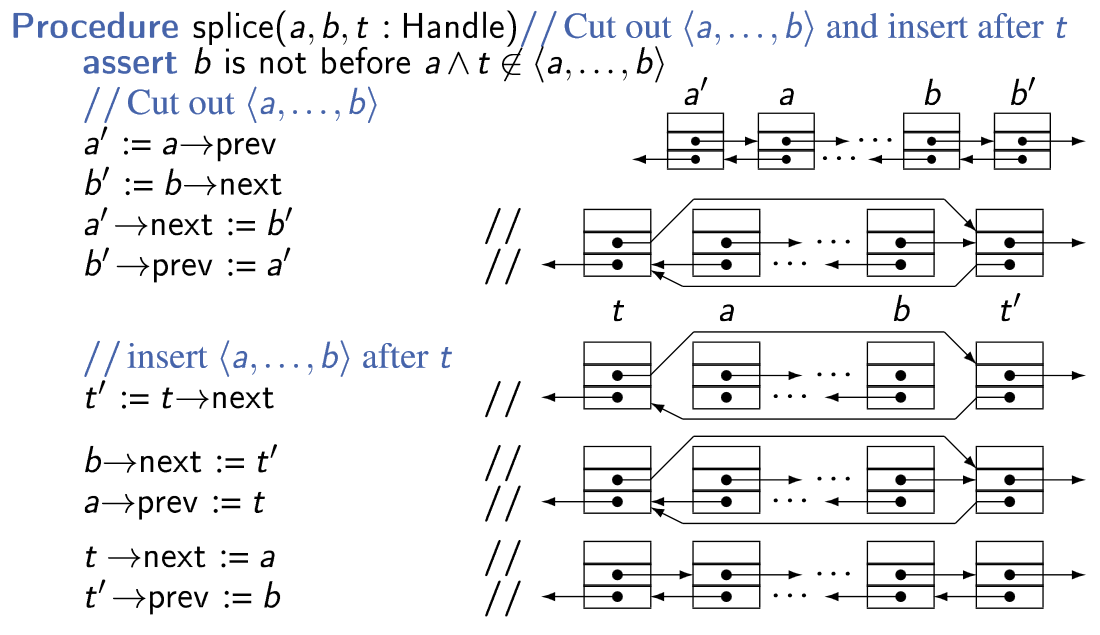
\includegraphics[height=7cm]{splice}
	\end{figure}
\end{frame}

% TODO Soll das rein? Siehe ÜB!
\begin{frame}{Verkettete Listen}
	\begin{exampleblock}{Anwendung: Konstruierung einer \emph{Unbounded Queue}}
		\LComment{Erinnerung: $\|splice|(a, b, t : \|Handle|)$ schneidet $\langle a,...,b \rangle$ aus} \\
		\LComment{seiner zugehörigen Liste aus und fügt es nach $t$ ein} \\
		\begin{tabular}{  p{5,5cm} c }
			\begin{algorithm}[H]
				\DontPrintSemicolon
				\footnotesize
				$head = \|createHandle|(\bot) : \|Handle|$\;
				\;
				\Procedure{pushBack$(e : \|Element|)$} {
					$new := \|createHandle|(e)$\;
					$new \access prev := new \access next := new$\;
					$\|splice|(new, new, head\access prev)$\;
				}
			\end{algorithm}
			&
			\begin{algorithm}[H]
				\DontPrintSemicolon
				\footnotesize
				\;
				\Function{popBack$ : \|Element|$} {
					$\KwAssert \neg isEmpty$\;
					$old := head \access prev$\;
					$e := old \access e$\;
					$d := \|createHandle|(\bot)$\;
					$d \access prev := d \access next := d$\;
					\;
					$\|splice|(old, old, d)$\;
					\;
					$\KwDispose old, d$\;
					\KwRet{$e$}\;
				}
			\end{algorithm}
		\end{tabular}
	\end{exampleblock}
\end{frame}

\begin{frame}{Verkettete Listen}
	\begin{exampleblock}{Anwendung: Konstruierung einer \emph{Unbounded Queue}}
		\LComment{Erinnerung: $splice(a, b, t : Handle)$ schneidet $\langle a,...,b \rangle$ aus} \\
		\LComment{seiner zugehörigen Liste aus und fügt es nach $t$ ein}
		\begin{tabular}{  p{5,5cm} c }
			\begin{algorithm}[H]
				\footnotesize
				$head = \|createHandle|(\bot) : \|Handle|$\;
				\;
				\Procedure{pushFront$(e : \|Element|)$} {
					$new := \|createHandle|(e)$\;
					$new \access prev := new \access next := new$\;
					$\|splice|(new, new, head)$\;
				}
			\end{algorithm}
			&
			\begin{algorithm}[H]
				\DontPrintSemicolon
				\footnotesize
				\;
				\Function{popFront$ : \|Element|$} {
					$\KwAssert \neg isEmpty$\;
					$old := head \access next$\;
					$e := old \access e$\;
					$d := \|createHandle|(\bot)$\;
					$d \access prev := d \access next := d$\;
					\;
					$\|splice|(old, old, d)$\;
					\;
					$\KwDispose old, d$\;
					\KwRet{$e$}\;
				}
			\end{algorithm}
		\end{tabular}
	\end{exampleblock}
\end{frame}


\begin{frame}{Verkettete Listen – Zweifel?}
	Arrays:  nur begrenzt toll \\
			 verkettete Listen: \textbf{unbegrenzt toll}? \quad (\#WorstPunEver)
	\pause
	\begin{itemize}
		\item[\Cons] List[i] nicht in $O(1)$, sondern linear
		\pause
		\item[\Cons] List.$size$ in $O(1)$ \; und gleichzeitig \; \textit{Inter-List-Splice}: \\
		Autsch
		\pause
		\item[\Cons] Cache-Freundlichkeit sieht anders aus
	\end{itemize}
\end{frame}

\begin{frame}{Einschub: Cache-Freundlichkeit}
	\begin{itemize}
		\item \textbf{Cache}: Prozessor-nahes Datenzwischenlager. Schneller als RAM.
		\pause
		\item \textbf{Lokalitätsprinzip}: Irgendwo Zugriff im RAM \impl demnächst wieder Zugriff in der Nähe
		\pause
		\implitem \textit{Idee}: Nicht nur \textbf{einen} Wert im Cache puffern, sondern dessen \textbf{Nachbarschaft} gleich mit! \\
		Kostet auch nicht mehr.
		\pause
		\item Verkettete Listen: Segmente \textbf{nach Bedarf} angelegt: \\ Landen da, wo's passt \impl \textbf{kreuz und quer} im RAM verteilt
		\pause 
		\implitem Vorgänger/Nachfolger sicher \textbf{nicht nebeneinander} \impl selten gemeinsam im Cache
		\pause
		\item Wie kriegen wir bloß Daten \textbf{zusammenhängend} in den Speicher?
		
		%\item Ein Cache „versteckt“ kürzlich abgerufene Werte aus dem Speicher in Prozessornähe
		%\pause
		%\item Ausnutzung des \textbf{Lokalitätsprinzips}: Wird ein Wert aus dem Speicher abgerufen, dann wird wahrscheinlich in zeitlicher Nähe ein Wert aus räumlicher Nähe abgerufen
		%\pause
		%\item Das Liefern der Nachbarschaft an den Cache ist kein echter Mehraufwand, da die meiste Zeit für den Datentransport benötigt wird (rein physikalische Beschränkung durch die Distanz zwischen Prozessor und Hauptspeicher)
		%\pause
		%\item Bei verketteten Listen werden Segmente nach Bedarf im Speicher allokiert, d.h. man kann nicht bestimmen, wo genau sie dann im Speicher liegen (meistens kreuz und quer verteilt). \\
		%\pause
		%\item Wenn es doch nur eine Möglichkeit gäbe, Elemente als zusammenhängenden Block im Speicher anzulegen ...
	\end{itemize}
\end{frame}

\section{...und Arrays (feat. amortisierte Analyse)}

\begin{frame}{Arrays to the rescue\only<1-2|handout:0>{?}\only<3->{!}}
	\begin{itemize}
		\item Array läuft voll \impl Größeres Array anlegen und Daten umkopieren
		\pause
		\item Naiv: Einfügen von $n$ Elementen in $\Theta(n^2)$
		\pause
		\item \textbf{Trick}: Jedes Mal ein doppelt so großes Array anlegen
		\item Ist das nicht trotzdem \textbf{teuer}!?
	\end{itemize}
\end{frame}

\begin{frame}{Amortisierte Analyse – a taste}
	\textbf{Einfügen} in ein \textbf{volles} Array (Größe $2n$):
	\begin{itemize}
		\implitem Array muss vergrößert (also umkopiert werden)
		\pause
		\item Genau \textbf{dieses} Einfügen kostet jetzt $2n$ (wegen Kopiererei)
		\pause
		\item \textbf{Vorher} mind. $n$ Einfüge-Operationen  in $O(1)$
		\pause
		\implitem \textbf{Amortisierte} Kopierkosten pro Einfügen: $\frac{2n}{n} = 2 \in O(1)$
	\end{itemize} \pause
	\forcenewline
	Genauso: \textbf{Entfernen} aus einem \textbf{viertel-vollen} Array ($n$ von $4n$ gefüllt)
	\begin{itemize} 
		\implitem Array muss verkleinert ($=$ umkopiert) werden
		\pause
		\item Genau \textbf{dieses} Entfernen kostet $n$ (wegen Kopiererei)
		\pause
		\item \textbf{Vorher} mind. $n$ Entfern-Operationen  in $O(1)$
		\pause
		\implitem \textbf{Amortisierte} Kopierkosten pro Entfernen: $\frac{n}{n} = 1 \in O(1)$
	\end{itemize}
\end{frame}

\begin{frame}{Amortisierte Analyse – How to}
	Entweder \\
	\textbf{Aggregatmethode}: Schätze nach oben ab:
	\[
		\text{Gesamtkosten von $n$ \textcolor{blue}{beliebigen} Ops} = \text{„}T_\text{Gesamt}\text{“} \ \leq \ c \cdot n 
	\]
	($c$ irgendeine Konstante). \\ \forcenewline
	Knifflig: Diese Abschätzung finden und zeigen.
\end{frame}

\begin{frame}{Amortisierte Analyse – How to}
	... oder \\
	\textbf{Kontomethode}: Kosten von teuren Operationen auf die billigen \textbf{umlegen} \\ \forcenewline 
	\pause
	\hanging Für jede Op der Art $i$: \quad  $c_i$ „Münzen“ auf ein „Konto“ einzahlen ($c_i$ \textbf{konstant}!) \\ 
	\pause
	\textcolor{blue}{Bsp}.: \hanging Arten von Ops \{Einfügen, Löschen\} \impl $c_\text{Einfügen}, c_\text{Löschen}$ festlegen \\
	\pause
	\hanging {Begründen: \newline Wenn mal eine Op \textbf{mehr als konstante Zeit} kostet (sagen wir $x$) \impl auf dem Konto mind. $x$ Münzen da, um das zu bezahlen.} \\
	\pause \forcenewline
	Knifflig: Begründen und die jeweiligen $c_i$ finden.
\end{frame}

\begin{frame}{Amortisierte Analyse – How to}
	\begin{itemize}
		\item \textbf{Generell}: Genau überlegen, unter welchen Vorbedingungen die teuren Operationen auftreten
		\item \textbf{Aufgabenstellung} beachten, ob spezifische Methode gefordert ist! (Falls nein \impl klare logische Begründung des Sachverhaltes reicht (im Prinzip))
	\end{itemize}
\end{frame}

\section{Aufgaben}

\begin{frame}{Amortisierte Analyse}
	\taskheading{Hochgestackte Ziele} 
	Gegeben seien zwei Stacks mit $size() : \N_0$, $pushBack(e : Element)$ und $popBack() : Element$, alle jeweils in konstanter Zeit. \\
	\smallskip
	Entwerft daraus eine Queue, die die Operationen $pushBack(e : Element)$ und $popFront() : Element$ jeweils in amortisiert konstanter Zeit beherrscht.
\end{frame}

\begin{frame}{Amortisierte Analyse}
	 \solutionheading
	\begin{itemize}
		\item ein „\textbf{Input}-Stack“, ein „\textbf{Output}-Stack“
		\item Queue.\textit{pushBack}: auf den Input-Stack legen
		\item Queue.\textit{popFront}: vom Output-Stack oben wegnehmen \\ 
		\pause
			  Output $= \emptyset$? \\
			  \impl Gesamten \textbf{Input}-Stack nach und nach auf Output \textbf{umschaufeln} (in $O(n)$). Dabei wird automatisch Reihenfolge richtigrum-gedreht. 
		\pause
		\item Queue.\textit{pushBack} sowieso in $O(1)$
		\pause
		\item Queue.\textit{popFront} hat \textbf{einmal} Kopieraufwand $n$, aber \textbf{danach} geht \textit{popFront} $n$-mal in $O(1)$ \\
		\pause
		\impl amortisiert in $O(1)$
	\end{itemize}
	% Verwende einen Stack als Input-Stack und einen Stack als Output-Stack, d.h. alle Elemente, die angehängt werden, werden auf den Input-Stack gelegt. Elemente, die entnommen werden, werden vom Output-Stack genommen, und falls dieser leer ist, wird in linearer Zeit der gesamte Inhalt vom Input-Stack auf den Output-Stack gelegt (die Reihenfolge wird dabei umgedreht, so dass das letzte Element vom Input-Stack das erste Element vom Output-Stack wird). $pushBack(e : Element)$ läuft immer in konstanter Zeit. Wenn $popFront()$ den Kopieraufwand $n$ hat, heißt das, dass danach n-mal $popFront()$ in konstanter Zeit funktionieren wird \\
	% $\Rightarrow$ amortisiert konstante Laufzeit.
\end{frame}




\begin{frame}{Amortisierte Analyse}
	\taskheading{A little bit more?} 
	Gegeben sei ein binärer Zähler mit einer unbegrenzten Anzahl an Bits, die alle auf 0 initialisiert sind. Der Zähler besitzt die Operation $increment$ (erhöht den im Zähler gespeicherten Wert um 1). \\ 
	\smallskip
	Ein einzelnes Bit zu flippen zählt jeweils als eine konstante Operation. Zeigt anhand der \textbf{Aggregatmethode}, dass die Operation \emph{increment} stets in amortisiert konstanter Zeit läuft.
\end{frame}

\begin{frame}{Amortisierte Analyse}
	\solutionheading \smallskip
	\textbf{Beobachtung}: \\
	Bit Nr. $i\ (i \geq 0)$ wird genau alle $2^i$ Aufrufe geflippt \\
	{\small \hanging (d.h. Bit Nr. 0 bei jedem Aufruf, Bit Nr. 1 alle zwei Aufrufe usw.)} \\
	\pause
	\impl im Schnitt wird Bit Nr. $i$ pro Aufruf $\frac{1}{2^i}$-mal geflippt \\
	\pause
	\impl im Schnitt haben $n$ Aufrufe von \textit{increment} die Kosten \[
		n \cdot \sum\limits_{i=0}^{M} \frac{1}{2^i} < n \cdot \sum\limits_{i=0}^{\infty} \frac{1}{2^i} = 2 \cdot n
	\] ($M$: Index des höchsten gesetzten Bits) \\
	\pause
	\impl läuft amortisiert in $O(1)$.
\end{frame}



\begin{frame}{Amortisierte Analyse}
	\taskheading{Bitte null Bit!} 
	Gegeben sei ein binärer Zähler mit einer unbegrenzten Anzahl an Bits, die alle auf 0 initialisiert sind. Der Zähler besitzt die Operationen $increment$ (erhöht den im Zähler gespeicherten Wert um 1) \textbf{und} $reset$ (setzt den im Zähler gespeicherten Wert auf 0 zurück). \\
	\smallskip
	Ein einzelnes Bit zu flippen zählt jeweils als eine konstante Operation. Zeigt anhand der \textbf{Kontomethode}, dass beide Methoden stets in amortisiert konstanter Zeit laufen.
\end{frame}

\begin{frame}{Amortisierte Analyse}
	\solutionheading \smallskip
	\textbf{Beobachtung}: 
	\begin{itemize}
		\item Bei jedem \emph{increment}-Aufruf: \\
			  \textbf{genau ein} Bit von $0 \rightsquigarrow 1 \Impl O(1)$ \\
			  u. U. \textbf{viele} Bits von $1 \rightsquigarrow 0 \Impl$ nicht-konstante Zeit
		\pause
		\item Bei jedem \emph{reset}-Aufruf: \\
			  u. U. \textbf{viele} Bits von $1 \rightsquigarrow 0 \Impl$ nicht-konstante Zeit
	\end{itemize}
	\pause
	%\textbf{Beobachtung}: Bei jedem Aufruf von $increment$ wird genau ein Bit von 0 auf 1 geflippt \impl Die nicht-konstanten Kosten von $increment$ und $reset$ entstehen durch die vielen 1er, die auf 0 gesetzt werden müssen. \\ 
	\textbf{Idee}: Jedes Mal wenn ein Bit von $0 \rightsquigarrow 1$ (pro Methodenaufruf max. $1$-mal!): $+1$ Münze einzahlen. Wenn das entspr. Bit wieder von $1 \rightsquigarrow 0$: Bezahle mit dieser Münze. \\
	\pause
	\impl Anzahl 1er im Zähler $=$ Anzahl Münzen auf dem Konto \\
	\pause
	\impl Bei beliebiger Op kann das Setzen von $n$ Bits von $1 \rightsquigarrow 0$ garantiert mit $n$ Münzen bezahlt werden. \\
	\pause
	\impl Beide Ops laufen amortisiert in $O(1)$.
	%\textbf{Idee}: Zahle jedes Mal, wenn eine 0 auf 1 geflippt wird (was pro Methodenaufruf max. 1-mal passiert), eine Münze aufs Konto ein. Bezahle mit dieser Münze, wenn das zugehörige Bit wieder auf 0 gesetzt wird. \\
	%Die Anzahl der 1er im Zähler repräsentiert also die Anzahl der Münzen auf dem Konto und garantiert somit, dass das Setzen von $n$ Bits von 1 auf 0 mit $n$ Münzen bezahlt werden kann. \\
	%\impl Amortisiert konstante Laufzeit beider Operationen.
\end{frame}



\begin{frame}{Datenstrukturen}
	\taskheading{Verrückte Datenstrukturen}
	Nehmt an, dass eine Speicherallokation beliebiger Größe in $O(1)$ läuft. Entwickelt eine Datenstruktur mit
	\begin{itemize}
		\item $pushBack(e : Element)$ und $popBack() : Element$ in $O(1)$ im Worst-Case (\textbf{nicht} nur amortisiert)
		\item Zugriff auf das $k$-te Element in $O(\log n)$ im Worst-Case (\textbf{nicht} nur amortisiert)
	\end{itemize}
\end{frame}

\begin{frame}{Datenstrukturen} % TODO Text überarbeiten
	\solutionheading
	Lege eine verkettete Liste von Arrays an, deren Größe sich jeweils verdoppelt, und habe immer eine Referenz auf das letzte Array inklusive Index des letzten belegten Slots
	\pause
	\begin{itemize}
		\item Element anfügen: Falls Slot frei \impl offensichtlich konstant. Falls kein Slot frei \impl lege neues Array doppelter Größe an, füge es an die verkettete Liste hinzu, lege Element rein (alles in konstanter Zeit möglich)
		\pause
		\item Zugriff auf das $k$-te Element: Laufe die verkettete Liste ab und verringere den Index um die Länge des aktuell betrachteten Arrays, bis der Index für das aktuell betrachtete Array gültig ist. Es sind insgesamt logarithmisch viele Arrays, also auch logarithmische Laufzeit
	\end{itemize}
\end{frame}



\begin{frame}{Datenstrukturen}
	\taskheading{Aufgabe~\the\numexpr\thetasknum-1\relax\ remastered} 
	Nehmt an, dass eine Speicherallokation beliebiger Größe in $O(1)$ läuft. Entwickelt eine Datenstruktur mit
	\begin{itemize}
		\item $pushBack(e : Element)$ und $popBack() : Element$ in $O(\log n)$ im Worst-Case (\textbf{nicht} nur amortisiert)
		\item Zugriff auf das $k$-te Element in $O(1)$ im Worst-Case (\textbf{nicht} nur amortisiert)
	\end{itemize}
\end{frame}

\begin{frame}{Datenstrukturen} % TODO Text überarbeiten
	\solutionheading
	Analog zur Lösung von Aufgabe 4: Lege ein Array $A$ mit Referenzen auf Arrays an, deren Größe sich jeweils verdoppelt (d.h. das Array an der Stelle $A[i]$ hat die Größe $2^i$)
	\pause
	\begin{itemize}
		\item Element anfügen: Falls Slot frei \impl offensichtlich konstant. Falls kein Slot frei \impl lege neues Array $B$ der Größe $2^{|A|}$ an, kopiere $A$ mit logarithmisch vielen Array-Referenzen in ein neues Array der Größe $|A|+1$ (an dessen Ende $B$ landet) und füge das Element in $B$ ein $\impl O(\log n)$
		\pause
		\item Zugriff auf das $k$-te Element: Berechne mit dem Logarithmus den Index von $B$ in $A$ und den Index des $k$-ten Elements in $B$, der Zugriff ist in konstanter Zeit.
	\end{itemize}
\end{frame}

\xkcdframe{379}{Danke für die Aufmerksamkeit! \smiley}{0}
% Alternativ: 163

\end{document}